% Copyright 2021 Politecnico di Milano, Italy. Inc. All rights reserved

\documentclass{PoliMi_MasterThesis}

% === Packages and configurations ===
% Configurations
\usepackage{parskip} % For paragraph layout
\usepackage{setspace} % For using single or double spacing
\usepackage{emptypage} % To insert empty pages
\setlength\parindent{0pt} % Indentation
\raggedbottom % Do not stretch empty space to fill the page

% Titles
\usepackage{titlesec}
% \titlespacing{\section}{left spacing}{before spacing}{after spacing}
\titlespacing{\section}{0pt}{3.3ex}{2ex}
\titlespacing{\subsection}{0pt}{3.3ex}{1.65ex}
\titlespacing{\subsubsection}{0pt}{3.3ex}{1ex}
\usepackage{color}

% Language and fonts
\usepackage[english]{babel} % The document is in English  
\usepackage[utf8]{inputenc} % UTF8 encoding
\usepackage[T1]{fontenc} % Font encoding
\usepackage[11pt]{moresize} % Big fonts

% Images
\usepackage{graphicx} % For images
\graphicspath{{./Images/}} % Directory of the images
\usepackage{transparent} % Enables transparent images
\usepackage{eso-pic} % For the background picture on the title page
\usepackage{subfig} % Numbered and caption subfigures using \subfloat.
\usepackage{tikz} % A package for high-quality hand-made figures.
\usetikzlibrary{}
\usepackage{caption} % Coloured captions
\usepackage{xcolor} % Coloured captions
\usepackage{amsthm,thmtools,xcolor} % Coloured "Theorem"
\usepackage{float}

% Math
\usepackage{amsmath}
\usepackage{amsthm}
\usepackage{amssymb}
\usepackage{amsfonts}
\usepackage{bm}
\usepackage[overload]{empheq} % For braced-style systems of equations.
\usepackage{fix-cm} % To override original LaTeX restrictions on sizes

% Tables
\usepackage{tabularx}
\usepackage{longtable} % Tables that can span several pages
\usepackage{colortbl}

% Algorithms
\usepackage{algorithm}
\usepackage{algorithmicx}
\usepackage{algpseudocodex}
\newcommand*\Let[2]{\State #1 $\gets$ #2}
\newcommand*\AAnd{\textbf{ and }}
\newcommand*\AOr{\textbf{ or }}

% Bibliography
\usepackage[colorlinks=true,linkcolor=black,anchorcolor=black,citecolor=black,filecolor=black,menucolor=black,runcolor=black,urlcolor=black]{hyperref} % Adds clickable links at references
\usepackage{cleveref}
\usepackage[square, numbers, sort&compress]{natbib} % Square brackets, citing references with numbers, citations sorted by appearance in the text and compressed
\bibliographystyle{abbrvnat} % You may use a different style adapted to your field

% Other packages
\usepackage{pdfpages} % To include a pdf file
\usepackage{afterpage}
\usepackage{fancyhdr} % For the headers
\fancyhf{}

% Input of configuration file. Do not change config.tex file unless you really know what you are doing. 
% Set the geometric layout of the document
\usepackage{geometry}
\geometry{
  top=3cm,
  left = 1.5cm,
  right = 1.5cm,
  bottom=2cm,
  headheight= 2cm,
  headsep= 0cm,
}
\raggedbottom 

% Create color bluePoli (-> manuale grafica coordinata:  https://www.polimi.it/fileadmin/user_upload/il_Politecnico/grafica-coordinata/2015_05_11_46xy_manuale_grafica_coordinata.pdf)
\definecolor{bluePoli}{cmyk}{0.4,0.1,0,0.4}

% Custom theorem environments
\declaretheoremstyle[
  headfont=\color{bluePoli}\normalfont\bfseries,
  bodyfont=\color{black}\normalfont\itshape,
]{colored}

\captionsetup[figure]{labelfont={color=bluePoli}} % Set colour of the captions
\captionsetup[table]{labelfont={color=bluePoli}} % Set colour of the captions
\captionsetup[algorithm]{labelfont={color=bluePoli}} % Set colour of the captions

\theoremstyle{colored}
\newtheorem{theorem}{Theorem}[section]
\newtheorem{proposition}{Proposition}[section]

% Enhances the features of the standard "table" and "tabular" environments.
\newcommand\T{\rule{0pt}{2.6ex}}
\newcommand\B{\rule[-1.2ex]{0pt}{0pt}}

% Algorithm description
\newcounter{algsubstate}
\renewcommand{\thealgsubstate}{\alph{algsubstate}}
\newenvironment{algsubstates}{
    \setcounter{algsubstate}{0}%
    \renewcommand{\STATE}{%
    \stepcounter{algsubstate}%
    \Statex {\small\thealgsubstate:}\space}
    }{}
    
% Custom theorem environment
\newcolumntype{L}[1]{>{\raggedright\let\newline\\\arraybackslash\hspace{0pt}}m{#1}}
\newcolumntype{C}[1]{>{\centering\let\newline\\\arraybackslash\hspace{0pt}}m{#1}}
\newcolumntype{R}[1]{>{\raggedleft\let\newline\\\arraybackslash\hspace{0pt}}m{#1}}

% Custom itemize environment
\setlist[itemize,1]{label=$\bullet$}
\setlist[itemize,2]{label=$\circ$}
\setlist[itemize,3]{label=$-$}
\setlist{nosep}

% Set separation of columns 
\setlength{\columnsep}{30pt}

% Create command for background pic
\newcommand\BackgroundPic{% Adding background picture
	\put(198,330){
		\parbox[b][\paperheight]{\paperwidth}{%
			\vfill
			\centering
			\transparent{0.4}
			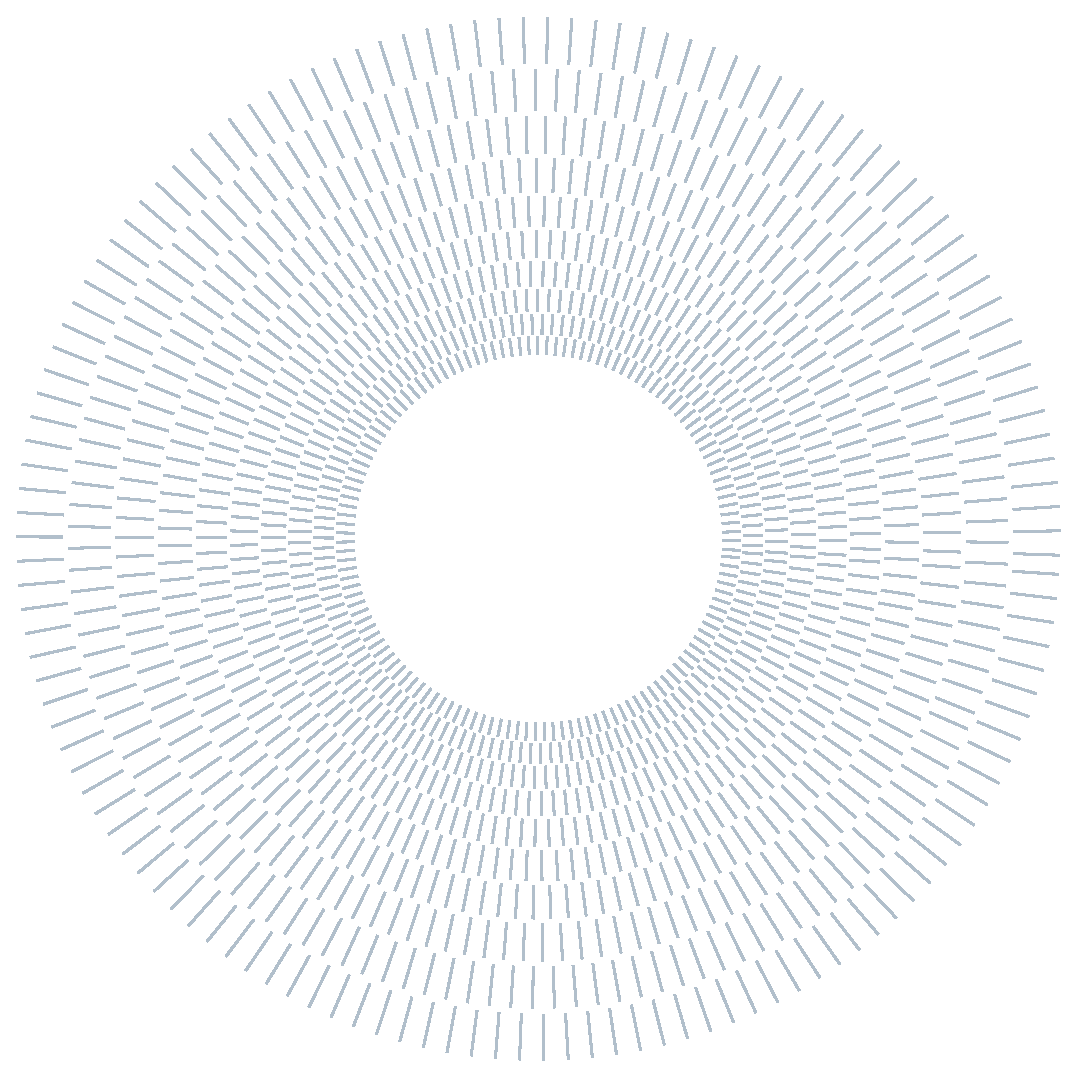
\includegraphics[width=0.7\paperwidth]{raggiera_polimi.eps}%
			\vfill
}}}

% Set indentation
\setlength\parindent{0pt}

% Custom title commands
\titleformat{\section}
{\color{bluePoli}\normalfont\Large\bfseries}
{\color{bluePoli}\thesection.}{1em}{}
\titlespacing*{\section}
{0pt}{2ex}{1ex}

\titleformat{\subsection}
{\color{bluePoli}\normalfont\large\bfseries}
{\color{bluePoli}\thesubsection.}{1em}{}
\titlespacing*{\subsection}
{0pt}{2ex}{1ex}

% Custom headers and footers
\pagestyle{fancy}
\fancyhf{}
      
\fancyfoot{}
\fancyfoot[C]{\thepage} % page
\renewcommand{\headrulewidth}{0mm} % headrule width
\renewcommand{\footrulewidth}{0mm} % footrule width

\makeatletter
\patchcmd{\headrule}{\hrule}{\color{black}\hrule}{}{} % headrule
\patchcmd{\footrule}{\hrule}{\color{black}\hrule}{}{} % footrule
\makeatother

% -> Create the header
\chead[C]{
\centering
\begin{tcolorbox}[arc=0pt, boxrule=0pt, colback=bluePoli!60, width=\textwidth, colupper=white]
    \textsc{\textbf{Executive summary}} \hfill \textsc{\textbf{\author}} 
\end{tcolorbox}
}


% === Start of document ===

\begin{document}

\fancypagestyle{plain}{
\fancyhf{} % Clear all header and footer fields
\fancyhead[RO,RE]{\thepage} %RO=right odd, RE=right even
\renewcommand{\headrulewidth}{0pt}
\renewcommand{\footrulewidth}{0pt}}


% === Title page ===
\pagestyle{empty} % No page numbers
\frontmatter % Use roman page numbering style (i, ii, iii, iv...) for the preamble pages

\puttitle{
	title=Ray Distribution Aware Heuristics for Bounding Volume Hierarchies Construction,
	name=Lapo Falcone,
	course=Computer Science and Engineering,
	ID  = 996089,
	advisor= Prof. Marco Gribaudo,
	academicyear={2023-24}
}


% === Preamble ===
\startpreamble
\setcounter{page}{1} % Set page counter to 1

% Abstract
\chapter*{Abstract} 
Abstract
\\
\\
\textbf{Keywords:} here, the keywords, of your thesis

% Abstract in Italian
\chapter*{Abstract in lingua italiana}
Abstract Italiano
\\
\\
\textbf{Parole chiave:} qui, vanno, le parole chiave, della tesi


% === Table of contents ===
\thispagestyle{empty}
\tableofcontents % Table of contents 
\thispagestyle{empty}
\cleardoublepage

\addtocontents{toc}{\vspace{2em}} % Add a gap in the Contents, for aesthetics
\mainmatter % Begin numeric (1,2,3...) page numbering


% === Intro ===
\chapter*{Introduction}
Intro \cite{meister2021survey}


% === Chapter 1 ===
\chapter{Chapter one}
\label{ch:chapter_one}
Chapter 1


% === Chapter 2 ... ===
\chapter{Chapter two}
Chapter 2


% === Bibliography ===
\addtocontents{toc}{\vspace{2em}} % Add a gap in the Contents, for aesthetics
\bibliography{Bibliography} % The references information are stored in the file named "Bibliography.bib"


% === Appendices ===
\cleardoublepage
\addtocontents{toc}{\vspace{2em}} % Add a gap in the Contents, for aesthetics
\appendix

\chapter{Collision and Culling Algorithms}
\section{Ray-AABB Intersection} \label{ray_box_intersection}
The algorithm we used to detect intersections between a ray and an AABB is the branchless slab algorithm \cite{ray_box_intersection}.
Given a ray in the form: $r(t) = O + t\cdot d$, where $O$ is the origin and $d$ the direction, the main idea of the algorithm is to find the 2 values of $t$ ($\overline{t_1}$ and $\overline{t_2}$) such that $r(\overline{t_{1,2}})$ are the points where the ray intersects the AABB.

Since the object to intersect the ray with is an axis-aligned bounding box in the min-max form, the algorithm can proceed one dimension at a time:
\begin{itemize}
	\item First, it finds the intersection points of the ray with the planes parallel to the $yz$ plane, and sorts them in an ascending order with reference to the corresponding $\overline{t_{1,2}}$ values.
	\item Then it does the same with the $xz$ plane:
	\begin{itemize}
		\item As closest intersection point, it keeps the furthest between the 2 closest intersection points found so far.
		\item As furthest intersection point, it keeps the closest between the 2 furthest intersection points found so far.
	\end{itemize}
	\item Then it does the same with the $xy$ plane.
	\item Finally, an intersection is detected only in the case where the furthest intersection point is actually further than the closest one found by the algorithm.
	\item The returned $\overline{t}$ value is the smaller one, as long as it is greater or equal to 0, otherwise it means that the origin of the ray is inside the AABB, and one of the intersection points is \textit{behind} the ray origin.
\end{itemize}
	
It is interesting to note how, under the floating-point IEEE 754 standard, the algorithm also works when it is not possible to find an intersection point along a certain axis (i.e. when the ray is parallel to certain planes). Indeed, in such cases, the values $\overline{t_{1,2}}$ will be $\pm \inf$, and the comparisons will still be well defined.


\begin{algorithm}[H]
	\caption{Ray-AABB branchless slab intersection algorithm in 3 dimensions}
	\begin{algorithmic}[1]
	\Function{Intersect}{$aabb, ray$}
	\Let {$tx1$}{$(aabb.min.x - ray.origin.x) / ray.direction.x$}
	\Let {$tx2$}{$(aabb.max.x - ray.origin.x) / ray.direction.x$}
	\Let {$tMin$}{$min(tx1, tx2)$}
	\Let {$tMax$}{$max(tx1, tx2)$}
	\Let {$ty1$}{$(aabb.min.y - ray.origin.y) / ray.direction.y$}
	\Let {$ty2$}{$(aabb.max.y - ray.origin.y) / ray.direction.y$}
	\Let {$tMin$}{$ max(tMin, min(ty1, ty2))$}
	\Let {$tMax$}{$ min(tMax, max(ty1, ty2))$}
	\Let {$tz1$}{$(aabb.min.z - ray.origin.z) / ray.direction.z$}
	\Let {$tz2$}{$(aabb.max.z - ray.origin.z) / ray.direction.z$}
	\Let {$tMin$}{$max(tMin, min(tz1, tz2))$}
	\Let {$tMax$}{$min(tMax, max(tz1, tz2))$}
	\Let {$areColliding$}{$tMax > tMin$ \AAnd $tMax \geq 0$}
	\Let {$collisionDist$}{$tMin < 0 ? tMax : tMin$}
	\State \Return $\langle areColliding, collisionDist \rangle$
	\EndFunction
	\end{algorithmic}
\end{algorithm} 

% === Lists ===
\listoffigures
\listoftables

% Table of symbols
\chapter*{List of Symbols} % You have to include a chapter for your list of symbols (
\begin{table}[H]
    \centering
    \begin{tabular}{lll}
        \textbf{Symbol} & \textbf{Description} & \textbf{Unit} \\\hline\\[-9px]
        $\bm{alpha}$ & symbol 1 & km \\[2px]
    \end{tabular}
\end{table}

% === Ringraziamenti ===
\chapter*{Acknowledgements}
Ringrazio...

\cleardoublepage
\end{document}
